\section{Predicting household power consumption using
RNN}\label{predicting-household-power-consumption-using-rnn}

\begin{lstlisting}[language=Python]
import torch
import torch.nn as nn
import numpy as np
import pandas as pd
import matplotlib.pyplot as plt
\end{lstlisting}

\begin{lstlisting}
/opt/venv/lib/python3.10/site-packages/tqdm/auto.py:21: TqdmWarning: IProgress not found. Please update jupyter and ipywidgets. See https://ipywidgets.readthedocs.io/en/stable/user_install.html
  from .autonotebook import tqdm as notebook_tqdm
\end{lstlisting}

The household power consumption dataset is taken from UCI Machine
Learning Repository. -
\href{https://archive.ics.uci.edu/ml/machine-learning-databases/00235/}{Data
Folder} -
\href{https://archive.ics.uci.edu/ml/datasets/individual+household+electric+power+consumption\#}{Data
Set Description}

\begin{lstlisting}[language=Python]
raw_data = pd.read_csv("../data/household_power_consumption.txt",
                       delimiter=";",
                       usecols=['Date', 'Time', 'Global_active_power'],
                       low_memory=False)
\end{lstlisting}

\begin{lstlisting}[language=Python]
def preprocess_data(df: pd.DataFrame) -> pd.DataFrame:
    # concatenante the "Date" and "Time" columns to create a "datetime" column
    # fix the data types of the "datetime" column and the "Global_active_power" column
    df = df.assign(
            datetime = lambda x: pd.to_datetime(x['Date'] + ' ' + x['Time']),
            Global_active_power = lambda x: pd.to_numeric(x['Global_active_power'], errors='coerce'),
        )
    df = df.dropna(subset=['Global_active_power'])
    df.sort_values(by='datetime', ascending=True, inplace=True)
    df = df.set_index("datetime")
    df.drop(['Date', 'Time'], axis=1, inplace=True)

    # normalize the data
    max_power = df['Global_active_power'].max()
    min_power = df['Global_active_power'].min()
    df['Global_active_power'] = (df['Global_active_power'] - min_power) / (max_power - min_power)
    return df, max_power, min_power

data, max_power, min_power = preprocess_data(raw_data)
data.tail()
\end{lstlisting}

Global\_active\_power

datetime

2010-12-11 23:55:00

0.055586

2010-12-11 23:56:00

0.055405

2010-12-11 23:57:00

0.055405

2010-12-11 23:58:00

0.055405

2010-12-11 23:59:00

0.055405

\begin{lstlisting}[language=Python]
# Visualize power for a day
date1 ='2009-05-08'
_ = data.loc[date1].plot(kind='line', y='Global_active_power', figsize=(10,6), grid=True)
plt.show()
plt.close()
\end{lstlisting}

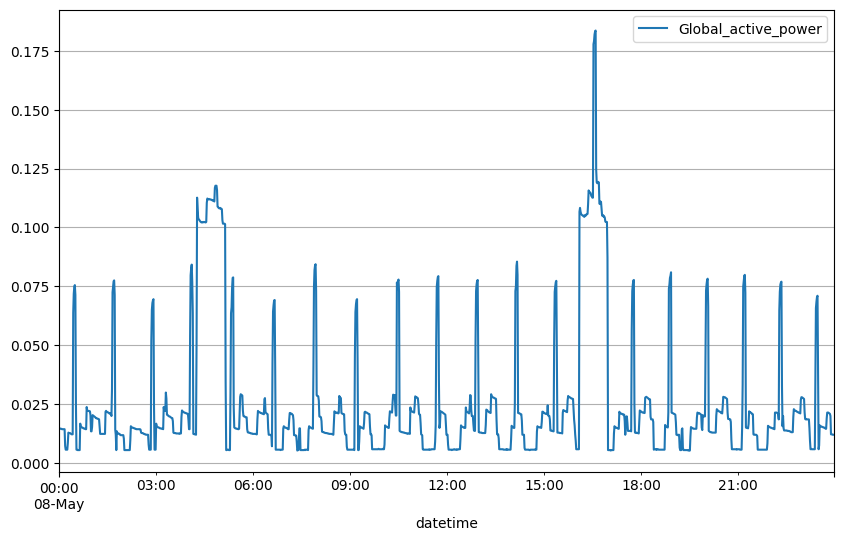
\includegraphics{img/rnn/intro/output_5_0_household.png}

\begin{lstlisting}[language=Python]
train_size = int(len(data) * 0.8)
train_data = data.iloc[:train_size].values
test_data = data.iloc[train_size:].values

def create_sequences(data, seq_len):
    """
    data: numpy array
        The input time series data
    seq_len: int
        The length of the input sequence
    """

    # initialize empty lists
    X = []
    y = []
    for i in range(seq_len, len(data)):
        X.append(data[i-seq_len:i])
        y.append(data[i])
    return np.array(X), np.array(y)

seq_len = 6   # number of past time steps to use for prediction, this is a hyperparameter

# Create train and test sequences
X_train, y_train = create_sequences(train_data, seq_len)
X_test, y_test = create_sequences(test_data, seq_len)

# convert numpy arrays to PyTorch tensors
X_train = torch.from_numpy(X_train).float()
y_train = torch.from_numpy(y_train).float()
X_test = torch.from_numpy(X_test).float()
y_test = torch.from_numpy(y_test).float()
\end{lstlisting}

\begin{lstlisting}[language=Python]
class RNN(nn.Module):
    def __init__(self, input_size, hidden_size, output_size):
        super(RNN, self).__init__()
        self.hidden_size = hidden_size
        self.rnn = nn.RNN(input_size, hidden_size, batch_first=True)
        self.fc = nn.Linear(hidden_size, output_size)

    def forward(self, x, hidden):
        out, hidden = self.rnn(x, hidden)
        out = self.fc(out[:, -1, :])
        return out, hidden
\end{lstlisting}

\textbf{Explanation}:

\begin{itemize}
\item
  First, the class is initialized with
  \lstinline{input\_size},
  \lstinline{hidden\_size}, and
  \lstinline{output\_size}. These parameters define the
  size of the input, hidden state, and output of the RNN.
\item
  The \lstinline{super(RNN, self).\_\_init\_\_()} line
  initializes the class as a subclass of the
  \lstinline{nn.Module} class in PyTorch, which provides
  some useful methods for defining and training neural networks.
\item
  The \lstinline{self.hidden\_size = hidden\_size} line
  sets the hidden size as an attribute of the class, so it can be
  accessed later in the forward method.
\item
  The \lstinline{nn.RNN} module is defined with the
  \lstinline{input\_size} and
  \lstinline{hidden\_size} parameters. The
  \lstinline{batch\_first=True} parameter indicates that
  the input to the RNN will have the batch dimension as the first
  dimension.
\item
  The \lstinline{nn.Linear} module is defined with the
  \lstinline{hidden\_size} and
  \lstinline{output\_size} parameters. This module will be
  used to map the final hidden state of the RNN to the output.
\item
  The forward method takes two arguments: \lstinline{x}
  and \lstinline{hidden}. \lstinline{x} is
  the input to the RNN, which is a tensor of shape
  \lstinline{(batch\_size, seq\_len, input\_size)}.
  \lstinline{hidden} is the initial hidden state of the
  RNN, which is a tensor of shape
  \lstinline{(1, batch\_size, hidden\_size)}.
\item
  The \lstinline{nn.RNN} module is called with
  \lstinline{x} and \lstinline{hidden} as
  inputs, and the output is stored in \lstinline{out}. The
  \lstinline{out} tensor has shape
  \lstinline{(batch\_size, seq\_len, hidden\_size)}, where
  \lstinline{seq\_len} is the length of the input
  sequence.
\item
  The \lstinline{out[:, -1, :]} indexing extracts the last
  hidden state of the RNN for each sequence in the batch. This tensor
  has shape \lstinline{(batch\_size, hidden\_size)}.
\item
  The \lstinline{nn.Linear} module is called with the last
  hidden state as input, and the output is stored in
  \lstinline{out}. The \lstinline{out}
  tensor has shape
  \lstinline{(batch\_size, output\_size)}.
\item
  Finally, the \lstinline{out} and
  \lstinline{hidden} tensors are returned as the output of
  the forward method.
\end{itemize}

Overall, this code defines a simple RNN model that takes an input
sequence, processes it with an RNN layer, and maps the final hidden
state to an output.

\subsubsection{Set Hyperparameters}\label{set-hyperparameters}

\begin{lstlisting}[language=Python]
input_size = 1   # number of features in the input
hidden_size = 32  # number of hidden units in the RNN layer
output_size = 1  # number of output features
learning_rate = 0.001
num_epochs = 100

# Tune the above hyperparameters for best results.

model = RNN(input_size, hidden_size, output_size)
criterion = nn.MSELoss()
optimizer = torch.optim.Adam(model.parameters(), lr=learning_rate)
\end{lstlisting}

\subsubsection{Training the model}\label{training-the-model}

\begin{lstlisting}[language=Python]
for epoch in range(num_epochs):
    # set the initial hidden state
    hidden = torch.zeros(1, X_train.size(0), hidden_size)

    # forward pass
    outputs, hidden = model(X_train, hidden)
    loss = criterion(outputs, y_train)

    # backwards and optimizer
    optimizer.zero_grad()
    loss.backward()
    optimizer.step()

    # Print loss at every 10th epoch
    if (epoch+1) % 10 == 0:
        print(f'Epoch [{epoch+1}/{num_epochs}], Loss: {round(loss.item(), 4)}')
\end{lstlisting}

\begin{lstlisting}
Epoch [10/100], Loss: 0.0145
Epoch [20/100], Loss: 0.0133
Epoch [30/100], Loss: 0.0093
Epoch [40/100], Loss: 0.009
Epoch [50/100], Loss: 0.0082
Epoch [60/100], Loss: 0.0077
Epoch [70/100], Loss: 0.0071
Epoch [80/100], Loss: 0.0065
Epoch [90/100], Loss: 0.0058
Epoch [100/100], Loss: 0.005
\end{lstlisting}

\textbf{Explanation}

\begin{itemize}
\item Loop through each epoch:
  \lstinline{for epoch in range(num\_epochs):} This loop
  iterates over the number of epochs specified in the num\_epochs
  variable.
\item Initialize the hidden state:
  \lstinline{hidden = torch.zeros(1, X\_train.size(0), hidden\_size)}
  The hidden state of the RNN is initialized to all zeros. The size of
  the tensor is \lstinline{(1, batch\_size, hidden\_size)}
  where \lstinline{batch\_size} is the number of samples
  in the training data and \lstinline{hidden\_size} is the
  number of hidden units in the RNN layer.
\item Forward pass:
  \lstinline{outputs, hidden = model(X\_train, hidden)}
  The RNN model is passed the input \lstinline{X\_train}
  and the initial hidden state hidden to generate the outputs and update
  the hidden state. The outputs tensor has shape
  \lstinline{(batch\_size, seq\_length, output\_size)}
  where \lstinline{seq\_length} is the length of the input
  sequence and \lstinline{output\_size} is the number of
  output features.
\item Calculate loss:
  \lstinline{loss = criterion(outputs, y\_train)} The loss
  is calculated based on the predicted outputs and the ground truth
  \lstinline{y\_train} using the mean squared error (MSE)
  loss.
\item Backward pass and optimizer step:
  \lstinline{optimizer.zero\_grad()     loss.backward()     optimizer.step()}
  The gradients of the model parameters are zeroed out, and the loss is
  backpropagated through the network. The optimizer then updates the
  model parameters based on the gradients.
\item Print loss:
  \begin{lstlisting}
      if (epoch+1) \% 10 == 0:
        print(f'Epoch [\{epoch+1\}/\{num\_epochs\}], Loss: \{round(loss.item(), 4)\}')
  \end{lstlisting}
  The loss is printed every 10th epoch using string formatting. The
  round function is used to round the loss to 4 decimal places.
\end{itemize}

\subsubsection{Model Evaluation}\label{model-evaluation}

\begin{lstlisting}[language=Python]
# Set initial hidden state for test data
hidden = torch.zeros(1, X_test.size(0), hidden_size)

# Forward pass
test_outputs, _ = model(X_test, hidden)

# Inverse normalize the output and inputs
test_outputs = (test_outputs * (max_power - min_power)) + min_power
y_test = (y_test * (max_power - min_power)) + min_power

# Compute the test loss
test_loss = criterion(test_outputs, y_test)

print(f'Test Loss: {round(test_loss.item(), 4)}')
\end{lstlisting}

\begin{lstlisting}
Test Loss: 0.4253
\end{lstlisting}

\begin{lstlisting}[language=Python]
# Convert the output and labels to numpy arrays
test_outputs = test_outputs.detach().numpy()
y_test = y_test.numpy()
# Plot the first 100 actual and predicted values
plt.plot(y_test[200:300], label='actual')
plt.plot(test_outputs[200:300], label='predicted')
plt.legend()
plt.show()
\end{lstlisting}

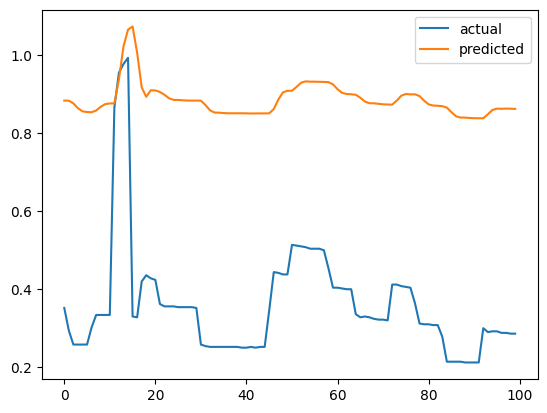
\includegraphics{img/rnn/intro/output_16_0_household.png}


\begin{lstlisting}[language=Python]
\end{lstlisting}
